\documentclass[12pt]{article}
\usepackage[table]{xcolor}
\usepackage[shortlabels]{enumitem}
\usepackage{tabularx,xltabular}
\usepackage{graphicx}
\usepackage{hyperref}
\usepackage{verbatim}
\usepackage{geometry}
\usepackage{ulem}
\usepackage[official]{eurosym}
\usepackage{tikz}
\usetikzlibrary{arrows,backgrounds,calc,decorations.markings,patterns,3d,positioning,fit,angles, quotes}
\usepackage{pgfplots}
\pgfplotsset{compat = newest}
\usetikzlibrary{fit}
\newcommand\addvmargin[1]{
\usetikzlibrary{arrows}
\node[fit=(current bounding box),inner ysep=#1,inner xsep=0]{};}
\usepackage{cancel}
\usepackage{fontspec}
\usepackage{array}  
\geometry{a4paper, top=2cm, left=2cm, right=2cm, bottom=2cm, headsep=1cm}
\usepackage{tabu}
\usepackage{pst-node}
\usepackage{colortbl}
\usepackage{array}
\usepackage{german}
\setlength\parindent{0pt}
\newcolumntype{?}{!{\vrule width 1pt}}
\usepackage{makecell}
\renewcommand{\arraystretch}{2.5}
\usepackage{pbox}
\usepackage{amssymb}
\usepackage{amsmath}
\usepackage{booktabs}
\newcolumntype{L}[1]{>{\raggedright\let\newline\\\arraybackslash\hspace{0pt}}m{#1}}
\newcolumntype{C}[1]{>{\centering\let\newline\\\arraybackslash\hspace{0pt}}m{#1}}
\newcolumntype{R}[1]{>{\raggedleft\let\newline\\\arraybackslash\hspace{0pt}}m{#1}}
\begin{document}
\rightline{Datum: 12.12.2023}
\centerline{{\Large Prozent und Zinsrechnung}} 
\vspace{1cm}
\noindent \\


\begin{xltabular}{\textwidth}{|C{0.75cm}|X|C{0.75cm}|X|}
\arrayrulecolor{black}\hline
a)&\pbox{5cm}{Wieviel Prozent sind schraffiert? \\
\tikzstyle{background grid}=[draw, black!15,step=.5cm]
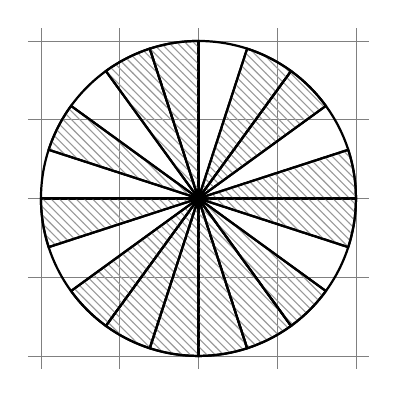
\begin{tikzpicture}[show background grid]
\pgfmathsetmacro{\R}{2}   
\draw[thick] (0,0) circle (\R); 
\draw[thick] (0,0) -- (90.0:\R);
\draw[thick] (0,0) -- (108.0:\R);
\draw[thick] (0,0) -- (126.0:\R);
\draw[thick] (0,0) -- (144.0:\R);
\draw[thick] (0,0) -- (162.0:\R);
\draw[thick] (0,0) -- (180.0:\R);
\draw[thick] (0,0) -- (198.0:\R);
\draw[thick] (0,0) -- (216.0:\R);
\draw[thick] (0,0) -- (234.0:\R);
\draw[thick] (0,0) -- (252.0:\R);
\draw[thick] (0,0) -- (270.0:\R);
\draw[thick] (0,0) -- (288.0:\R);
\draw[thick] (0,0) -- (306.0:\R);
\draw[thick] (0,0) -- (324.0:\R);
\draw[thick] (0,0) -- (342.0:\R);
\draw[thick] (0,0) -- (360.0:\R);
\draw[thick] (0,0) -- (378.0:\R);
\draw[thick] (0,0) -- (396.0:\R);
\draw[thick] (0,0) -- (414.0:\R);
\draw[thick] (0,0) -- (432.0:\R);
\draw[thick,pattern=north west lines, pattern color=black!40] (0,0) -- (360.0:\R) arc (360.0:378.0:\R) -- (0,0);
\draw[thick,pattern=north west lines, pattern color=black!40] (0,0) -- (108.0:\R) arc (108.0:126.0:\R) -- (0,0);
\draw[thick,pattern=north west lines, pattern color=black!40] (0,0) -- (396.0:\R) arc (396.0:414.0:\R) -- (0,0);
\draw[thick,pattern=north west lines, pattern color=black!40] (0,0) -- (234.0:\R) arc (234.0:252.0:\R) -- (0,0);
\draw[thick,pattern=north west lines, pattern color=black!40] (0,0) -- (288.0:\R) arc (288.0:306.0:\R) -- (0,0);
\draw[thick,pattern=north west lines, pattern color=black!40] (0,0) -- (144.0:\R) arc (144.0:162.0:\R) -- (0,0);
\draw[thick,pattern=north west lines, pattern color=black!40] (0,0) -- (180.0:\R) arc (180.0:198.0:\R) -- (0,0);
\draw[thick,pattern=north west lines, pattern color=black!40] (0,0) -- (342.0:\R) arc (342.0:360.0:\R) -- (0,0);
\draw[thick,pattern=north west lines, pattern color=black!40] (0,0) -- (414.0:\R) arc (414.0:432.0:\R) -- (0,0);
\draw[thick,pattern=north west lines, pattern color=black!40] (0,0) -- (90.0:\R) arc (90.0:108.0:\R) -- (0,0);
\draw[thick,pattern=north west lines, pattern color=black!40] (0,0) -- (306.0:\R) arc (306.0:324.0:\R) -- (0,0);
\draw[thick,pattern=north west lines, pattern color=black!40] (0,0) -- (216.0:\R) arc (216.0:234.0:\R) -- (0,0);
\draw[thick,pattern=north west lines, pattern color=black!40] (0,0) -- (252.0:\R) arc (252.0:270.0:\R) -- (0,0);
\draw[thick,pattern=north west lines, pattern color=black!40] (0,0) -- (270.0:\R) arc (270.0:288.0:\R) -- (0,0);
\end{tikzpicture}
}
&
b)&\pbox{5cm}{Wieviel Prozent sind schraffiert?\\
\tikzstyle{background grid}=[draw, black!15,step=.5cm]
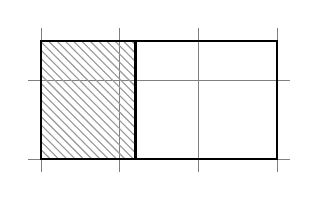
\begin{tikzpicture}[show background grid]
\pgfmathsetmacro{\laenge}{3}  
\pgfmathsetmacro{\hoehe}{\laenge/2}  
\pgfmathsetmacro{\percent}{40/100}  
\draw[thick] (0,0) rectangle ++ (\laenge,\hoehe);
\draw[thick,pattern=north west lines, pattern color=black!40] (0,0) rectangle ++ (\laenge*\percent,\hoehe);
\end{tikzpicture}
}
\\\hline
c)&Grundwert~500~kg;  Prozentsatz~5~\%
&
d)&Grundwert~500~g;  Prozentwert~10~g
\\\hline
e)&Prozentwert~4~Schüler;  Prozentsatz~1~\%
&
f)&Kapital~9.000~€;  Zinssatz~2~\%
\\\hline
g)&Kapital~8.760~€;  Zinsen~219~€
&
h)&Zinsen~150~€;  Zinssatz~5~\%
\\\hline
i)&Berechne die Monatszinsen für 6 Monate und $K=5.800~€$ bei $p~\%=5~\%$.
&
j)&Berechne das ersparte Geld nach 4 Jahren für K=550 € und p\%=2 \%
\\\hline
k)&645 - 296 = 
&
l)&93 + 548 = 
\\\hline
\end{xltabular}
\vspace{0.5cm}
\newpage
\rightline{Datum: 12.12.2023}
\centerline{{\large Lösungen Prozent und Zinsrechnung}} 
\vspace{0.5cm}

\begin{xltabular}{\textwidth}{|C{0.75cm}|X|C{0.75cm}|X|}
\arrayrulecolor{black}\hline
a)&$$\frac{14}{20}=0,7=70\%$$
&
b)&\pbox{5cm}{
\tikzstyle{background grid}=[draw, black!15,step=.5cm]
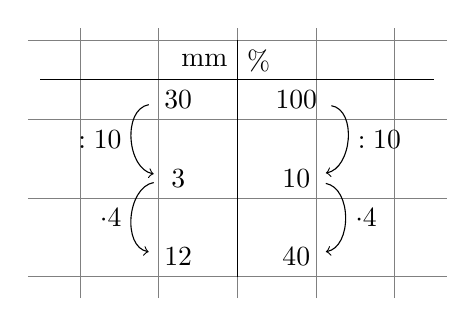
\begin{tikzpicture}[show background grid]
\draw[black] (0cm,0cm) -- (0cm,-3cm); 
\draw[black] (-2.5 cm,-0.5cm) -- (2.5cm,-0.5cm); 
\node[left] at (0 cm,-0.25cm) {mm};
\node[right] at (0 cm,-0.255cm) {\%};
\node[circle] (1) at (-0.75 cm,-0.75cm) {30};
\node[circle] (2) at (-0.75 cm,-1.75cm) {3};
\node[circle] (3) at (-0.75 cm,-2.75cm) {12};
\node[circle] (4) at (0.75 cm,-0.75cm) {100};
\node[circle] (5) at (0.75 cm,-1.75cm) {10};
\node[circle] (6) at (0.75 cm,-2.75cm) {40};
\draw[->] (1) to [out=190,in=170] node[left] {$:10$}  (2) ;
\draw[->] (2) to [out=190,in=170] node[left] {$\cdot 4$}  (3) ;
\draw[->] (4) to [out=350,in=10] node[right] {$:10$}  (5) ;
\draw[->] (5) to [out=350,in=10] node[right] {$\cdot4$}  (6) ;
\end{tikzpicture}
\newline
Oder: \newline
Gesamtlänge: 30\,mm, Länge der Schraffur: 12\,mm. Das bedeutet: \newline
$\frac{12}{30}=0,4=40\%$
}
\\\hline
c)&
\begingroup\setlength{\jot}{0.02cm}
\tikzstyle{background grid}=[draw, black!15,step=.5cm]
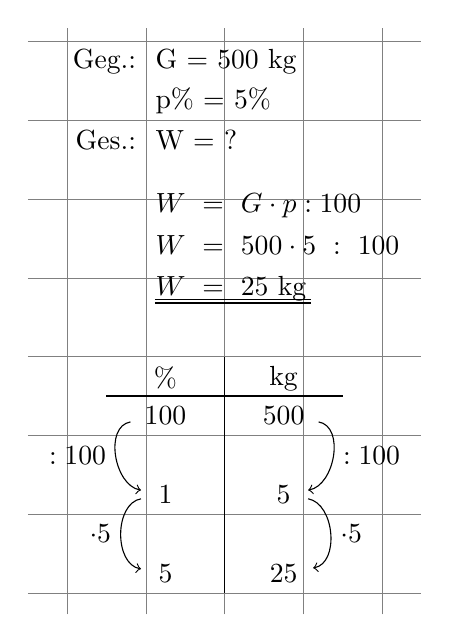
\begin{tikzpicture}[show background grid]
\node[left] at (0,-0.25) {Geg.: };
\node[right] at (0,-0.25) {G = 500 kg};
\node[right] at (0,-0.75) {p\% = 5\%};
\node[left] at (0,-1.-0.25) {Ges.: };
\node[right] at (0,-1.-0.25) {W  = ? };
\node[below right] at (0,-1.75) {
$\begin{aligned}
W\ &=\ G\cdot p : 100 \\
W\ &=\ 500\cdot 5\ :\ 100 \\
\makebox[0pt][l]{\uuline{\phantom{W\%\ =\ 25\ \mbox{kg}}}}
W\ &=\ 25\ \mbox{kg}
\end{aligned}$};

\draw[black] (1cm,-4cm) -- (1cm,-7cm); 
\draw[black] (-0.5 cm,-4.5cm) -- (2.5cm,-4.5cm); 
\node[below] at (0.25 cm,-4cm) {\%};
\node[below] at  (1.75 cm,-4cm) {kg};
\node[circle] (1) at (0.25 cm,-4.75cm) {100};
\node[circle] (2) at (0.25 cm,-5.75cm) {1};
\node[circle] (3) at (0.25 cm,-6.75cm) {5};
\node[circle] (4) at (1.75 cm,-4.75cm) {500};
\node[circle] (5) at (1.75 cm,-5.75cm) {5};
\node[circle] (6) at (1.75 cm,-6.75cm) {25};
\draw[->] (1) to [out=190,in=170] node[left] {$:100$}  (2) ;
\draw[->] (2) to [out=190,in=170] node[left] {$\cdot 5$}  (3) ;
\draw[->] (4) to [out=350,in=10] node[right] {$:100$}  (5) ;
\draw[->] (5) to [out=350,in=10] node[right] {$\cdot5$}  (6) ;
\end{tikzpicture}
\endgroup
&
d)&
\begingroup\setlength{\jot}{0.02cm}
\tikzstyle{background grid}=[draw, black!15,step=.5cm]
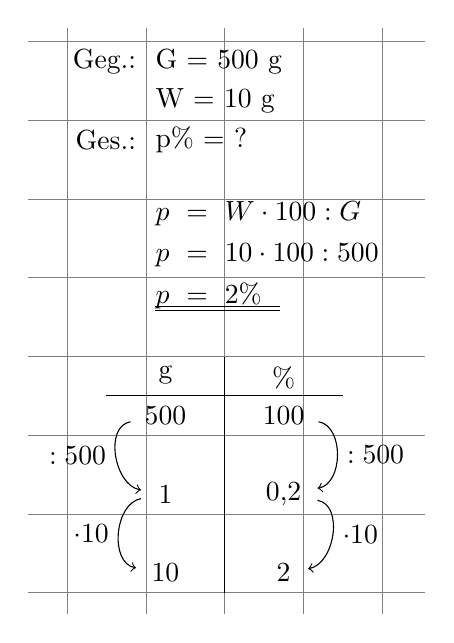
\begin{tikzpicture}[show background grid]
\node[left] at (0,-0.25) {Geg.: };
\node[right] at (0,-0.25) {G = 500 g};
\node[right] at (0,-0.75) {W = 10 g};
\node[left] at (0,-1.25) {Ges.: };
\node[right] at (0,-1.25) {p\%  = ? };
\node[below right] at (0,-1.85) {
$\begin{aligned}
p\ &=\ W\cdot 100 : G \\
p\ &=\ 10\cdot 100 : 500\ \\
\makebox[0pt][l]{\uuline{\phantom{p\%\ =\ 2\% }}}
p\ &=\ 2\% 
\end{aligned}$};

\draw[black] (1cm,-4cm) -- (1cm,-7cm); 
\draw[black] (-0.5 cm,-4.5cm) -- (2.5cm,-4.5cm); 
\node[below] at (0.25 cm,-4cm) {g};
\node[below] at  (1.75 cm,-4cm) {\%};
\node[circle] (1) at (0.25 cm,-4.75cm) {500};
\node[circle] (2) at (0.25 cm,-5.75cm) {1};
\node[circle] (3) at (0.25 cm,-6.75cm) {10};
\node[circle] (4) at (1.75 cm,-4.75cm) {100};
\node[circle] (5) at (1.75 cm,-5.75cm) {0,2};
\node[circle] (6) at (1.75 cm,-6.75cm) {2};
\draw[->] (1) to [out=190,in=170] node[left] {$:500$}  (2) ;
\draw[->] (2) to [out=190,in=170] node[left] {$\cdot 10$}  (3) ;
\draw[->] (4) to [out=350,in=10] node[right] {$:500$}  (5) ;
\draw[->] (5) to [out=350,in=10] node[right] {$\cdot10$}  (6) ;
\end{tikzpicture}
\endgroup
\\\hline
e)&
\begingroup\setlength{\jot}{0.02cm}
\tikzstyle{background grid}=[draw, black!15,step=.5cm]
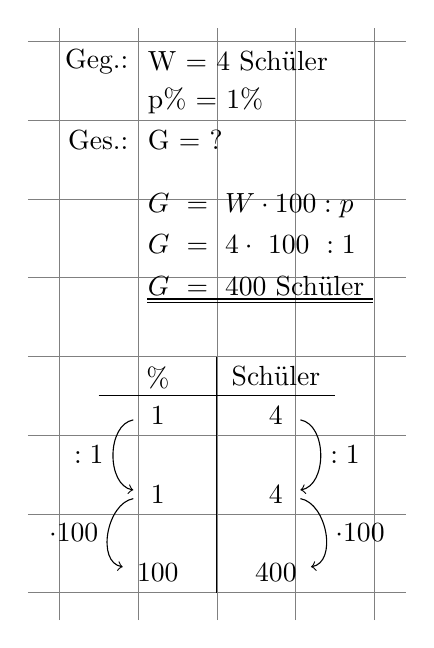
\begin{tikzpicture}[show background grid]
\node[left] at (0,-0.25) {Geg.: };
\node[right] at (0,-0.25) {W = 4 Schüler};
\node[right] at (0,-0.75) {p\% = 1\%};
\node[left] at (0,-1.-0.25) {Ges.: };
\node[right] at (0,-1.-0.25) {G  = ? };
\node[below right] at (0,-1.75) {
$\begin{aligned}
G\ &=\ W\cdot 100 : p \\
G\ &=\ 4\cdot\ 100\ :1 \\
\makebox[0pt][l]{\uuline{\phantom{G\%\ =\ 400\ \mbox{Schüler}}}}
G\ &=\ 400\ \mbox{Schüler}
\end{aligned}$};

\draw[black] (1cm,-4cm) -- (1cm,-7cm); 
\draw[black] (-0.5 cm,-4.5cm) -- (2.5cm,-4.5cm); 
\node[below] at (0.25 cm,-4cm) {\%};
\node[below] at  (1.75 cm,-4cm) {Schüler};
\node[circle] (1) at (0.25 cm,-4.75cm) {1};
\node[circle] (2) at (0.25 cm,-5.75cm) {1};
\node[circle] (3) at (0.25 cm,-6.75cm) {100};
\node[circle] (4) at (1.75 cm,-4.75cm) {4};
\node[circle] (5) at (1.75 cm,-5.75cm) {4};
\node[circle] (6) at (1.75 cm,-6.75cm) {400};
\draw[->] (1) to [out=190,in=170] node[left] {$:1$}  (2) ;
\draw[->] (2) to [out=190,in=170] node[left] {$\cdot 100$}  (3) ;
\draw[->] (4) to [out=350,in=10] node[right] {$:1$}  (5) ;
\draw[->] (5) to [out=350,in=10] node[right] {$\cdot100$}  (6) ;
\end{tikzpicture}
\endgroup
&
f)&
\begingroup\setlength{\jot}{0.02cm}
\tikzstyle{background grid}=[draw, black!15,step=.5cm]
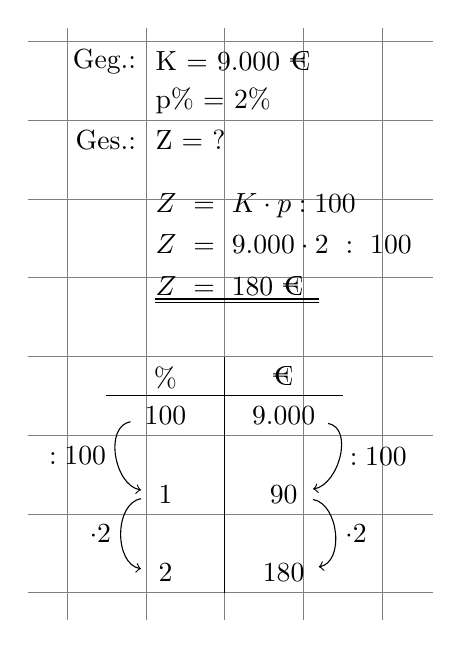
\begin{tikzpicture}[show background grid]
\node[left] at (0,-0.25) {Geg.: };
\node[right] at (0,-0.25) {K = 9.000 €};
\node[right] at (0,-0.75) {p\% = 2\%};
\node[left] at (0,-1.-0.25) {Ges.: };
\node[right] at (0,-1.-0.25) {Z  = ? };
\node[below right] at (0,-1.75) {
$\begin{aligned}
Z\ &=\ K\cdot p : 100 \\
Z\ &=\ 9.000\cdot 2\ :\ 100 \\
\makebox[0pt][l]{\uuline{\phantom{W\%\ =\ 180\ \mbox{€}}}}
Z\ &=\ 180\ \mbox{€}
\end{aligned}$};

\draw[black] (1cm,-4cm) -- (1cm,-7cm); 
\draw[black] (-0.5 cm,-4.5cm) -- (2.5cm,-4.5cm); 
\node[below] at (0.25 cm,-4cm) {\%};
\node[below] at  (1.75 cm,-4cm) {€};
\node[circle] (1) at (0.25 cm,-4.75cm) {100};
\node[circle] (2) at (0.25 cm,-5.75cm) {1};
\node[circle] (3) at (0.25 cm,-6.75cm) {2};
\node[circle] (4) at (1.75 cm,-4.75cm) {9.000};
\node[circle] (5) at (1.75 cm,-5.75cm) {90};
\node[circle] (6) at (1.75 cm,-6.75cm) {180};
\draw[->] (1) to [out=190,in=170] node[left] {$:100$}  (2) ;
\draw[->] (2) to [out=190,in=170] node[left] {$\cdot 2$}  (3) ;
\draw[->] (4) to [out=350,in=10] node[right] {$:100$}  (5) ;
\draw[->] (5) to [out=350,in=10] node[right] {$\cdot2$}  (6) ;
\end{tikzpicture}
\endgroup
\\\hline
g)&
\begingroup\setlength{\jot}{0.02cm}
\tikzstyle{background grid}=[draw, black!15,step=.5cm]
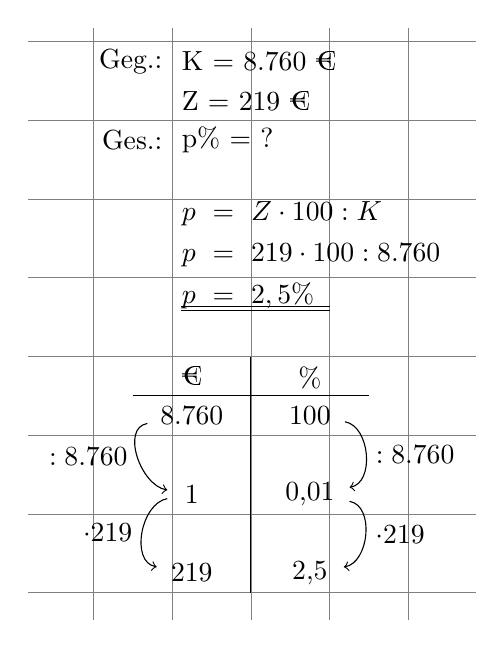
\begin{tikzpicture}[show background grid]
\node[left] at (0,-0.25) {Geg.: };
\node[right] at (0,-0.25) {K = 8.760 €};
\node[right] at (0,-0.75) {Z = 219 €};
\node[left] at (0,-1.25) {Ges.: };
\node[right] at (0,-1.25) {p\%  = ? };
\node[below right] at (0,-1.85) {
$\begin{aligned}
p\ &=\ Z\cdot 100 : K \\
p\ &=\ 219\cdot 100 : 8.760\ \\
\makebox[0pt][l]{\uuline{\phantom{p\%\ =\ 2,5\% }}}
p\ &=\ 2,5\% 
\end{aligned}$};

\draw[black] (1cm,-4cm) -- (1cm,-7cm); 
\draw[black] (-0.5 cm,-4.5cm) -- (2.5cm,-4.5cm); 
\node[below] at (0.25 cm,-4cm) {€};
\node[below] at  (1.75 cm,-4cm) {\%};
\node[circle] (1) at (0.25 cm,-4.75cm) {8.760};
\node[circle] (2) at (0.25 cm,-5.75cm) {1};
\node[circle] (3) at (0.25 cm,-6.75cm) {219};
\node[circle] (4) at (1.75 cm,-4.75cm) {100};
\node[circle] (5) at (1.75 cm,-5.75cm) {0,01};
\node[circle] (6) at (1.75 cm,-6.75cm) {2,5};
\draw[->] (1) to [out=190,in=170] node[left] {$:8.760$}  (2) ;
\draw[->] (2) to [out=190,in=170] node[left] {$\cdot 219$}  (3) ;
\draw[->] (4) to [out=350,in=10] node[right] {$:8.760$}  (5) ;
\draw[->] (5) to [out=350,in=10] node[right] {$\cdot219$}  (6) ;
\end{tikzpicture}
\endgroup
&
h)&
\begingroup\setlength{\jot}{0.02cm}
\tikzstyle{background grid}=[draw, black!15,step=.5cm]
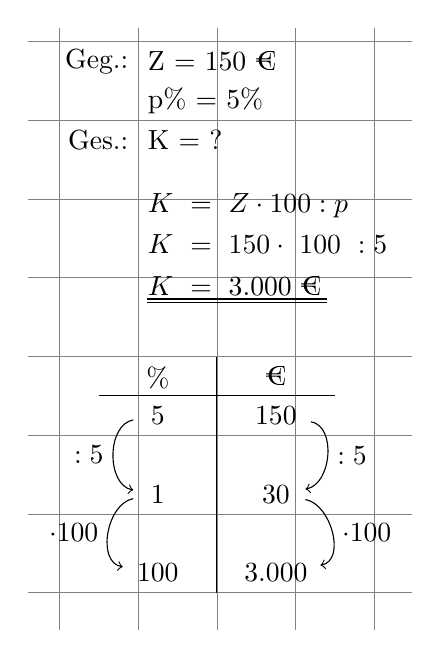
\begin{tikzpicture}[show background grid]
\node[left] at (0,-0.25) {Geg.: };
\node[right] at (0,-0.25) {Z = 150 €};
\node[right] at (0,-0.75) {p\% = 5\%};
\node[left] at (0,-1.-0.25) {Ges.: };
\node[right] at (0,-1.-0.25) {K  = ? };
\node[below right] at (0,-1.75) {
$\begin{aligned}
K\ &=\ Z\cdot 100 : p \\
K\ &=\ 150\cdot\ 100\ :5 \\
\makebox[0pt][l]{\uuline{\phantom{G\%\ =\ 3.000\ \mbox{€}}}}
K\ &=\ 3.000\ \mbox{€}
\end{aligned}$};

\draw[black] (1cm,-4cm) -- (1cm,-7cm); 
\draw[black] (-0.5 cm,-4.5cm) -- (2.5cm,-4.5cm); 
\node[below] at (0.25 cm,-4cm) {\%};
\node[below] at  (1.75 cm,-4cm) {€};
\node[circle] (1) at (0.25 cm,-4.75cm) {5};
\node[circle] (2) at (0.25 cm,-5.75cm) {1};
\node[circle] (3) at (0.25 cm,-6.75cm) {100};
\node[circle] (4) at (1.75 cm,-4.75cm) {150};
\node[circle] (5) at (1.75 cm,-5.75cm) {30};
\node[circle] (6) at (1.75 cm,-6.75cm) {3.000};
\draw[->] (1) to [out=190,in=170] node[left] {$:5$}  (2) ;
\draw[->] (2) to [out=190,in=170] node[left] {$\cdot 100$}  (3) ;
\draw[->] (4) to [out=350,in=10] node[right] {$:5$}  (5) ;
\draw[->] (5) to [out=350,in=10] node[right] {$\cdot100$}  (6) ;
\end{tikzpicture}
\endgroup
\\\hline
i)&
\pbox{5cm}{
$\begin{aligned}
geg.: K&=5.800 € \\
   p\%&=5 \% \\
ges.: Z_{6M}&=? \\
 Z&=K\cdot p\% \\
 Z&=5.800\cdot 0,05 \\
 Z&=290 €\\
 Z_{1M}&=290 € : 12\\
 Z_{1M}&=24,17 €\\
 Z_{6M}&=24,17 € \cdot 6\\
\makebox[0pt][l]{\uuline{\phantom{$ Z_{6M}=145 €\\$} } }
 Z_{6M}&=145 €\\
\end{aligned}$ \\
}
&
j)&\pbox{5cm}{
Nach 1 Jahren: \\
$\begin{aligned}
Z_1&=K_{start}\cdot p\% \\
&=550 € \cdot 0,02 \\
&=11 €\\
K_1&=K_{start}+Z \\
&=550 €+ 11 €\\
\makebox[0pt][l]{\uuline{\phantom{$K_1=561 €\\$} } }
K_1&=561 €\\
\end{aligned}$ \\
Nach 2 Jahren: \\
$\begin{aligned}
Z_2&=K_1\cdot p\% \\
&=561 € \cdot 0,02 \\
&=11,22 €\\
K_2&=K_1+Z \\
&=561 €+ 11,22 €\\
\makebox[0pt][l]{\uuline{\phantom{$K_2=572,22 €\\$} } }
K_2&=572,22 €\\
\end{aligned}$ \\
Nach 3 Jahren: \\
$\begin{aligned}
Z_3&=K_2\cdot p\% \\
&=572,22 € \cdot 0,02 \\
&=11,44 €\\
K_3&=K_2+Z \\
&=572,22 €+ 11,44 €\\
\makebox[0pt][l]{\uuline{\phantom{$K_3=583,66 €\\$} } }
K_3&=583,66 €\\
\end{aligned}$ \\
Nach 4 Jahren: \\
$\begin{aligned}
Z_4&=K_3\cdot p\% \\
&=583,66 € \cdot 0,02 \\
&=11,67 €\\
K_4&=K_3+Z \\
&=583,66 €+ 11,67 €\\
\makebox[0pt][l]{\uuline{\phantom{$K_4=595,34 €\\$} } }
K_4&=595,34 €\\
\end{aligned}$ \\
}
\\\hline
k)&645 - 296 = 349
&
l)&93 + 548 = 641
\\\hline
\end{xltabular}
\vspace{0.5cm}
\end{document}